\documentclass[11pt]{article}

\usepackage[margin=1in]{geometry}
\usepackage{graphicx}
\usepackage{amsmath}
\usepackage{hyperref}
\usepackage{listings}
\usepackage{xcolor}
\usepackage{booktabs}
\usepackage{enumitem}
\usepackage[T1]{fontenc}
\usepackage{tikz}
\usetikzlibrary{positioning, arrows.meta, fit, backgrounds, calc}

\hypersetup{
  colorlinks=true,
  linkcolor=blue!60!black,
  citecolor=blue!60!black,
  urlcolor=blue!60!black
}

\lstset{
  basicstyle=\ttfamily\small,
  backgroundcolor=\color{gray!8},
  frame=single,
  framerule=0.4pt,
  rulecolor=\color{gray!40},
  breaklines=true,
  breakatwhitespace=true,
  columns=fullflexible,
  keepspaces=true,
  showstringspaces=false,
  keywordstyle=\color{blue!70!black},
  commentstyle=\color{green!50!black},
  stringstyle=\color{red!60!black},
  xleftmargin=1em,
  xrightmargin=1em,
  aboveskip=0.8em,
  belowskip=0.8em,
}

\lstdefinelanguage{yaml}{
  keywords={true,false,null},
  morecomment=[l]{\#},
  morestring=[b]',
  morestring=[b]",
}

\title{DSAgt: A Compartmentalized Agent Toolkit\\
       for AI-Ready Scientific Data Pipelines}
\author{
  Aaron Tuor\thanks{Pacific Northwest National Laboratory},
  Rohith A.\ Varikoti\footnotemark[1],
  Nestor Demeure\thanks{Lawrence Berkeley National Laboratory},
  Andrew Tritt\footnotemark[2],\\
  Jean Luca Bez\footnotemark[2],
  Jong Youl Choi\thanks{Oak Ridge National Laboratory},
  Kyle Parfrey\thanks{Princeton Plasma Physics Laboratory},
  Shreyas Cholia\footnotemark[2]
}
\date{}

\begin{document}
\maketitle

%% ----------------------------------------------------------------
%% Abstract
%% ----------------------------------------------------------------

\begin{abstract}
DSAgt (DataSmith Agent) provides an AI agent with two
MCP servers---a tool and skill registry and a knowledge
base---together supporting the construction of scientific
data processing pipelines.
The agent registers domain-specific CLI tools at runtime,
discovers instruction-based skills for complex workflows,
consults indexed documentation to inform processing decisions,
and executes tools directly via shell with automatic
provenance capture.
A local LLM proxy captures structured conversation traces
that feed an episodic memory system and enable pipeline
reconstruction from execution records.
All project state---configuration, tools, skills, knowledge
collections, execution traces, memory, and observability
data---lives in a single self-contained project directory.
The architecture imposes no pipeline taxonomy and no platform
lock-in: any MCP-compatible agent works with the same servers.
We describe the design and walk through a worked example using
microbial isolate sequencing data.
\end{abstract}

%% ----------------------------------------------------------------
%% 1  Introduction
%% ----------------------------------------------------------------

\section{Introduction}

Building AI-ready datasets from raw scientific data requires
domain-specific processing, quality assessment, and metadata
standardization.
These requirements differ across domains---time-series sensor
data, electron micrographs, and spectroscopic measurements
each demand different tools, quality criteria, and validation
logic.

A common approach is to define a fixed taxonomy of pipeline
stages (ingestion, cleaning, validation, transformation,
export), each implemented as a software component with a
prescribed interface.
In practice, scientific processing does not decompose cleanly
along these lines.
A genomic quality filter may evaluate base quality scores,
adapter contamination, and read length simultaneously---it is
validation, filtering, and reporting at once.
When processing steps do not map to the taxonomy, code written
to satisfy it accumulates unnecessary abstractions: adapter
classes, stage registries, and inter-stage schemas that serve
the framework rather than the work.

DSAgt takes a different approach.
It provides two server-side capabilities---a registry for
tools and skills, and semantic search over indexed
documentation---exposed as MCP servers, plus a project
lifecycle managed through a single CLI.
The same servers support a human-in-the-loop chat session
where the agent proposes and executes steps interactively,
a fully autonomous pipeline, or a structured workflow with
explicit stage control.
What varies across these modes is the agent implementation
and its guidance, not the servers or tools.

Several design commitments follow.
The servers communicate over MCP stdio and import no agent
SDK, so switching agent implementations requires only changing
the \texttt{agent} field in the project configuration.
DSAgt defines no pipeline stages---a tool has a name, takes
parameters, and produces output; sequencing is determined by
the agent.
Tool execution happens at the shell level, giving the agent
direct access to return codes, stderr, and standard Unix
process controls.
A single YAML configuration file is the source of truth for
API keys, endpoints, and settings; DSAgt's code reads the
configuration and sets environment variables for downstream
processes, eliminating reliance on shell profile exports.

%% ----------------------------------------------------------------
%% 2  Architecture
%% ----------------------------------------------------------------

\section{Architecture}

DSAgt consists of two MCP servers, a project lifecycle CLI,
a LiteLLM proxy for observability, and a memory system
(Figure~\ref{fig:architecture}).
All project state lives in a single self-contained directory
created by \texttt{dsagt init} and managed through the
\texttt{dsagt} CLI.

\paragraph{Project Lifecycle.}
\texttt{dsagt init <name> -{}-agent <platform>} creates a
project directory (defaulting to
\texttt{\textasciitilde/dsagt-projects/<name>/}) containing
the configuration file, subdirectories for tools, skills,
knowledge collections, execution traces, and MLflow data.
Projects are registered in
\texttt{\textasciitilde/.dsagt/projects.yaml} so that
\texttt{dsagt start <name>} works from any directory.
On start, DSAgt generates platform-specific agent
configuration files from a single master instruction set,
starts the LiteLLM proxy and MLflow, and launches the agent
CLI.
When the agent exits, memory extraction runs automatically
and services are stopped.

\paragraph{Tool Execution and Provenance.}
Each registered tool is a markdown file with YAML frontmatter
containing the machine-readable specification (name,
description, executable, parameters, dependencies, tags) and
a markdown body with usage guidance.
When a tool is registered via \texttt{save\_tool\_spec}, the
executable is automatically wrapped with \texttt{dsagt-run}
for provenance capture and \texttt{uv run -{}-with} for
Python dependency isolation.
The agent reads the tool file and executes the wrapped command
directly via shell.
\texttt{dsagt-run} captures the exact command, return code,
stdout/stderr, timing, and file I/O as a structured JSON
record in the project's trace archive.
Concurrently, the LiteLLM proxy callback captures the agent's
tool call intent and reported outcome, producing three-layer
provenance records: intent from the proxy, execution from the
wrapper, and report from the proxy.

\paragraph{Tools and Skills.}
DSAgt distinguishes two types of registered capabilities.
\emph{Tools} are CLI executables with parameters, stored as
markdown files in the project's \texttt{tools/} directory.
\emph{Skills} are instruction-based agent workflows---a
\texttt{SKILL.md} file with a workflow definition plus
optional reference documents---stored in the project's
\texttt{skills/} directory.
Both are indexed into ChromaDB collections at registration
time for semantic search and metadata filtering.
The agent discovers tools via \texttt{search\_registry}
and skills via \texttt{search\_skills}, which support exact
name lookup, tag filtering, and natural-language semantic
search.
DSAgt ships with a bundled \texttt{datacard-generator} skill
for MODCON Datacard v1 documentation.

\paragraph{Registry Server.}
The registry server enables the agent to discover, register,
and search for tools and skills.
It can read local files, fetch documentation from URLs,
execute shell commands (typically \texttt{-{}-help}), save
tool specifications, install Python dependencies, and
reconstruct pipelines from execution records.
The \texttt{reconstruct\_pipeline} tool renders the session's
tool call sequence as a reproducible bash script or Snakemake
workflow by analyzing input/output file overlap across
execution records.

\paragraph{Knowledge Base.}
The knowledge base provides semantic search over indexed
document collections.
Collections can use FAISS or ChromaDB as the vector backend,
with per-collection routing that allows different embedding
models and backends to coexist.
\texttt{kb\_ingest} indexes a folder as a new collection;
\texttt{kb\_append} adds files to an existing collection.
Pre-built collections (e.g., NeMo Curator and AIDRIN
documentation) are symlinked into the project at startup.
The same search interface serves domain documentation,
episodic memory, registered tools, and registered skills.

\paragraph{Memory System.}
Routing provenance, prior tool executions, and accumulated
session knowledge through vector-indexed collections rather
than the agent's working context is central to DSAgt's
design.
A naive agent loop accumulates every tool call, output, and
intermediate artifact in-context, which makes long or
iterative scientific workflows quickly exceed the model's
context window and degrades reasoning quality well before
that limit.
By persisting tool execution records, episodic facts, and
domain documents into queryable ChromaDB collections, DSAgt
keeps the live context small while preserving a complete,
auditable trail that the agent can retrieve on demand.
This separation also makes the same store usable for
post-hoc auditing of agent behavior and for reconstructing
reproducible pipelines from arbitrarily long sessions.
DSAgt maintains two forms of agent-authored memory on top of
this substrate, both queryable through the knowledge base
search interface.
\emph{Episodic memory}: at session end (or triggered by
exchange volume), an LLM call extracts facts, a session
summary, and cross-fact insights from the session log.
These are stored in the \texttt{episodic\_memory} ChromaDB
collection with categorical metadata.
A centroid-based outlier detection mechanism flags unusual
facts for user review.
\emph{Explicit memory}: the agent can store user-confirmed
facts via \texttt{kb\_remember}, which writes to a YAML file
loaded into agent context at session start.

\paragraph{Observability.}
All LLM calls route through a local LiteLLM proxy that
captures two streams: OpenTelemetry spans (token counts,
latency, cost) exported to a per-project MLflow instance, and
DSAgt tool execution records written to the trace archive.
MLflow provides a web UI for inspecting token usage, latency,
and full request/response traces.

\paragraph{Agent Guidance.}
A single master instruction file
(\texttt{dsagt\_instructions.md}) defines the agent's
behavioral guidance: tool preference hierarchy, iterative
workflow, knowledge base usage patterns, and tool generation
conventions.
At project start, this file is automatically formatted for
the target platform---appended to \texttt{CLAUDE.md} for
Claude Code, written as \texttt{.goosehints} for Goose,
converted to a JSON \texttt{.roomodes} file for Roo Code,
or placed in \texttt{.clinerules/} for Cline.
Four CLI-based agent platforms are supported: Claude Code,
Goose, Roo Code, and Cline.

%% ----------------------------------------------------------------
%% Figure 1: Architecture
%% ----------------------------------------------------------------

\begin{figure}[t]
\centering
\resizebox{\textwidth}{!}{%
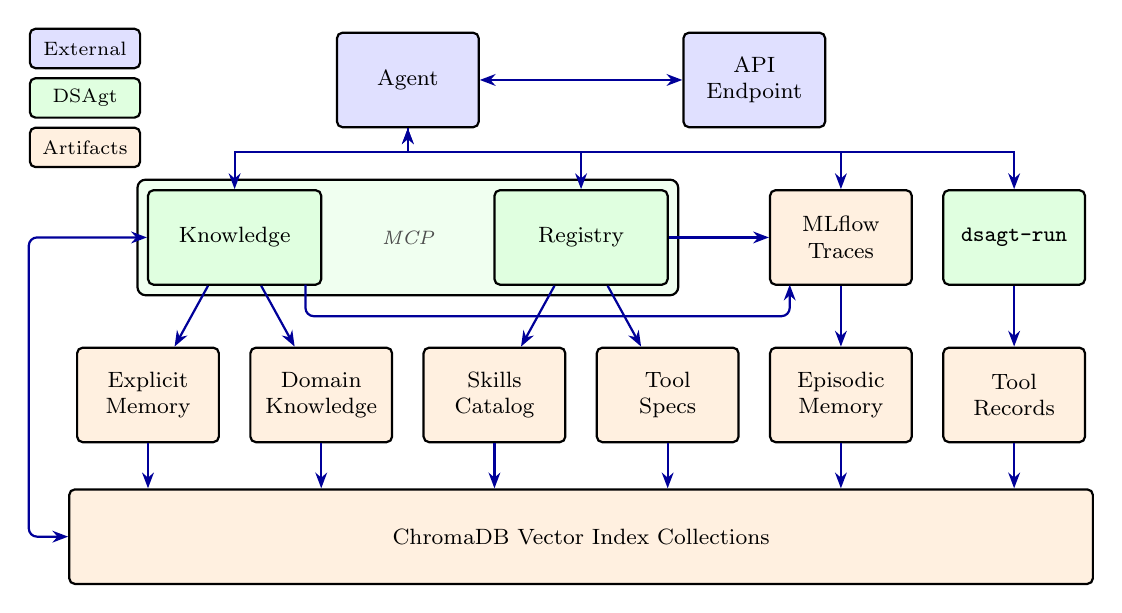
\begin{tikzpicture}[
    >={Stealth[length=2mm]},
    box/.style={
        draw, rounded corners=2pt, thick,
        minimum width=22mm, minimum height=12mm,
        align=center, font=\footnotesize,
        fill=white},
    ext/.style={box, fill=blue!12},          % External Provider
    svc/.style={box, fill=green!12},         % DSAgt Services
    art/.style={box, fill=orange!12,         % Project Artifacts
                minimum width=18mm},
    db/.style={draw, rounded corners=2pt, thick,
               fill=orange!12, align=center,
               font=\footnotesize,
               minimum height=12mm},
    link/.style={->, thick, blue!60!black},
    bilink/.style={<->, thick, blue!60!black},
    lbl/.style={font=\scriptsize\itshape, text=gray!60!black},
]

% ===== Legend (left of Agent) =====
% Left edge aligned with the Knowledge<->ChromaDB vertical run at
% x=-3.5.  Legend width is 14mm = 1.4 units, so center sits at
% x=-3.5 + 0.7 = -2.8.
\node[ext, minimum width=14mm, minimum height=5mm,
      font=\scriptsize] (leg1) at (-2.8, 0.4)
  {External};
\node[svc, minimum width=14mm, minimum height=5mm,
      font=\scriptsize, below=1mm of leg1]
  (leg2) {DSAgt};
\node[art, minimum width=14mm, minimum height=5mm,
      font=\scriptsize, below=1mm of leg2]
  (leg3) {Artifacts};

% ===== Row 1: Agent <-> API =====
% Row 3 collections are placed on a uniform 2.2-unit grid (see Row 3
% comment); every other row's x-coordinates are derived from that grid.
% Agent is centered between Knowledge (-0.9) and Registry (3.5) at x=1.3.
% API is symmetric around the figure's central column at x=3.5, landing
% at x=5.7.  Both boxes narrowed to 18mm to match the artifact row.
\node[ext, minimum width=18mm] (agent) at (1.3,0) {Agent};
\node[ext, minimum width=18mm] (api)   at (5.7,0) {API\\Endpoint};

\draw[bilink] (agent) -- (api);

% ===== Row 2: MCP servers + MLflow + dsagt-run =====
% Knowledge centered above (Explicit, Domain); Registry above (Skills,
% Tool Specs); MLflow directly above Episodic; dsagt-run directly above
% Tool Records.  All x-coordinates fall out of the row-3 grid below.
\node[svc] (knowledge) at (-0.9,-2) {Knowledge};
\node[svc] (registry)  at (3.5,-2)  {Registry};
\node[art] (mlflow)    at (6.8,-2)  {MLflow\\Traces};
% dsagt-run width matches the artifact boxes (18mm) so it visually
% pairs with MLflow Traces and Tool Records on either side.
\node[svc, minimum width=18mm] (dsagtrun) at (9.0,-2) {\texttt{dsagt-run}};

% The Knowledge and Registry tool surfaces are now exposed by ONE merged
% MCP server (dsagt-server).  A single container box spans + sits behind
% both (background layer, lighter fill) so the two inner boxes still read
% as distinct concern modules while the bridge conveys "one server".
\begin{scope}[on background layer]
  \node[draw, rounded corners=3pt, thick, fill=green!6,
        fit=(knowledge)(registry), inner sep=1.2mm] (mcpbox) {};
\end{scope}

% Agent <-> MCP servers (symmetric forks; bidirectional because MCP is
% request/response — the server replies travel back to the agent).
\draw[bilink] (agent.south) -- ++(0,-0.3) -| (knowledge.north);
\draw[bilink] (agent.south) -- ++(0,-0.3) -| (registry.north);
% MCP label in the center of the merged-server box, in the gap between the
% Knowledge and Registry modules — the bridge that joins them into one server.
\node[lbl] at (1.3,-2) {MCP};

% Agent -> MLflow + dsagt-run (fork off the same trunk as the MCP servers,
% drop vertically directly above each box).
\draw[link] (agent.south) -- ++(0,-0.3) -| (mlflow.north);
\draw[link] (agent.south) -- ++(0,-0.3) -| (dsagtrun.north);

% Registry -> MLflow (direct horizontal hop, same row)
\draw[link] (registry.east) -- (mlflow.west);

% Knowledge -> MLflow (routed under row 2 to avoid the registry box).
% Stem x=0.0 = right of the knowledge->domain diagonal (which exits
% knowledge.south near x=-0.57) but still inside the Knowledge Server's
% south edge (spans x=-2.0 to x=0.2).
% End-stem x=6.15 = on MLflow's south edge, offset left of the
% mlflow->episodic arrow at x=6.8 to avoid overlap.
% Horizontal run y=-3 = midway between row 2 (y=-2) and row 3 (y=-4).
\draw[link, rounded corners=3pt]
  (0.0,-2.6) -- (0.0,-3) -- (6.15,-3) -- (6.15,-2.6);

% ===== Row 3: Collections =====
% Six artifact boxes on a uniform 2.2-unit grid (left edge to left edge):
% Explicit Memory, Domain Knowledge, Skills, Tool Specs, Episodic Memory,
% Tool Records.  Knowledge MCP server feeds Explicit Memory via
% kb_remember; dsagt-run wrapper writes Tool Records to the trace archive
% on every registered-tool invocation.
\node[art] (explicit) at (-2.0,-4) {Explicit\\Memory};
\node[art] (domain)   at (0.2,-4)  {Domain\\Knowledge};
\node[art] (skills)   at (2.4,-4)  {Skills\\Catalog};
\node[art] (tools)    at (4.6,-4)  {Tool\\Specs};
\node[art] (episodic) at (6.8,-4)  {Episodic\\Memory};
\node[art] (history)  at (9.0,-4)  {Tool\\Records};

% Knowledge -> explicit memory (kb_remember) and domain knowledge
\draw[link] (knowledge) -- (explicit);
\draw[link] (knowledge) -- (domain);

% Registry -> skills and tool specs
\draw[link] (registry) -- (skills);
\draw[link] (registry) -- (tools);

% MLflow -> episodic memory
\draw[link] (mlflow) -- (episodic);

% dsagt-run -> Tool Records (vertical drop, mirrors MLflow -> Episodic)
\draw[link] (dsagtrun) -- (history);

% ===== Row 4: ChromaDB bus =====
% Centered at x=3.5 (the row-3 midpoint) and 130mm wide so chroma.west
% lands exactly at x=-3.0, where the knowledge<->chroma bend already
% terminates (no spurious final hop).
\node[db, minimum width=130mm] (chroma) at (3.5,-5.8)
  {ChromaDB Vector Index Collections};

\foreach \n in {domain, skills, tools, episodic,
                history, explicit} {
    \draw[link] (\n) -- (\n |- chroma.north);
}

% Knowledge <-> ChromaDB (bidirectional, bent left — clear path).
% Bend offset is -1.5 (not -1.0) so the path's final horizontal segment
% into chroma.west has nonzero length; otherwise the |- operator would
% land on top of chroma.west with no clear direction for the arrowhead.
\draw[bilink, rounded corners=3pt]
  (knowledge.west) -- ++(-1.5,0) |- (chroma.west);

\end{tikzpicture}%
}% end resizebox
\caption{%
  DSAgt architecture.
  The agent communicates directly with the LLM API endpoint;
  its native OpenTelemetry exporter writes traces to a
  per-project MLflow store, and the \texttt{dsagt-run}
  tool wrapper records each tool invocation to the trace
  archive.
  Two MCP servers handle knowledge base search and explicit
  memory writes (left) and tool/skill registration (right).
  Six independently partitioned ChromaDB collections hold
  explicit memory, domain knowledge, skills, tool specs,
  episodic memory, and tool records, each with its own
  embedding backend and vector-DB route.
  The knowledge server dispatches queries to the appropriate
  collection and applies optional cross-encoder reranking
  to returned chunks.}
\label{fig:architecture}
\end{figure}

%% ----------------------------------------------------------------
%% 3  Worked Example: Microbial Isolate Processing
%% ----------------------------------------------------------------

\section{Worked Example: Microbial Isolate Processing}

We walk through a microbial isolate processing workflow using
short-read sequencing data from the NERSC amsc002 project,
consisting of paired-end FASTQ files for multiple bacterial
isolates.
Figure~\ref{fig:workflow} shows the sequence of interactions.

The workflow begins with project initialization:

\begin{lstlisting}[language=bash]
dsagt init isolate-pipeline --agent claude-code
vim ~/dsagt-projects/isolate-pipeline/dsagt_config.yaml
dsagt start isolate-pipeline
\end{lstlisting}

\noindent
The agent then operates within the project directory, with
MCP servers connected and the proxy capturing traces.

%% ----------------------------------------------------------------
%% Figure 2: Microbial Isolate Workflow
%% ----------------------------------------------------------------

\begin{figure}[t]
\centering
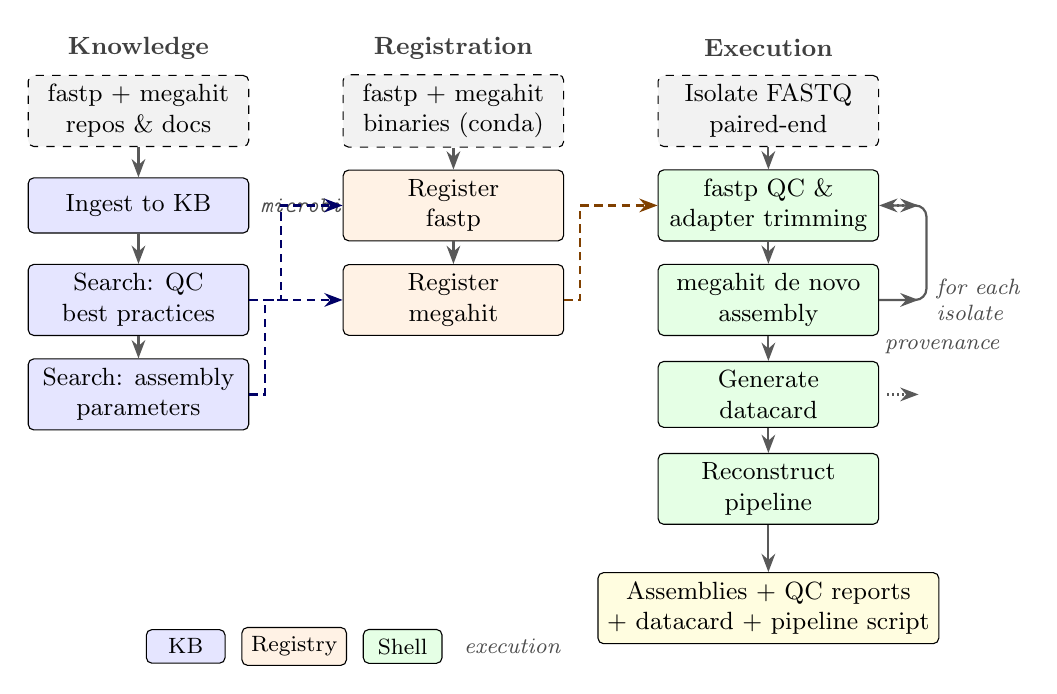
\begin{tikzpicture}[
    >=Stealth,
    node distance=0.5cm and 0.4cm,
    stp/.style={
      draw, rounded corners=2pt,
      minimum height=0.7cm, minimum width=2.8cm,
      align=center, font=\small},
    kb/.style={stp, fill=blue!10},
    reg/.style={stp, fill=orange!10},
    pipe/.style={stp, fill=green!10},
    inp/.style={stp, fill=gray!10, dashed},
    arr/.style={->, thick, gray!70!black},
    lbl/.style={font=\footnotesize\itshape,
                text=gray!60!black},
    phase/.style={font=\small\bfseries,
                  text=gray!50!black},
]

% Column positions
\def\colA{0}
\def\colB{4.0}
\def\colC{8.0}

% Phase headers
\node[phase] at (\colA, 0) {Knowledge};
\node[phase] at (\colB, 0) {Registration};
\node[phase] at (\colC, 0) {Execution};

% --- Knowledge column ---
\node[inp] (repos) at (\colA, -0.8)
  {fastp + megahit\\repos \& docs};
\node[kb]  (ingest)  at (\colA, -2.0)
  {Ingest to KB};
\node[kb]  (search1) at (\colA, -3.2)
  {Search: QC\\best practices};
\node[kb]  (search2) at (\colA, -4.4)
  {Search: assembly\\parameters};

\draw[arr] (repos) -- (ingest);
\draw[arr] (ingest)  -- (search1);
\draw[arr] (search1) -- (search2);

\node[lbl, right=0.02cm of ingest,  anchor=west]
  {\texttt{microbial\_isolates}};

% --- Registration column ---
\node[inp] (bins)  at (\colB, -0.8)
  {fastp + megahit\\binaries (conda)};
\node[reg] (regfastp) at (\colB, -2.0)
  {Register\\fastp};
\node[reg] (regmegahit) at (\colB, -3.2)
  {Register\\megahit};

\draw[arr] (bins)  -- (regfastp);
\draw[arr] (regfastp) -- (regmegahit);

% KB informs registration
\draw[arr, densely dashed, blue!40!black]
  (search1.east) -- ++(0.4,0) |- (regfastp.west);
\draw[arr, densely dashed, blue!40!black]
  (search2.east) -- ++(0.2,0) |- (regmegahit.west);

% --- Execution column ---
\node[inp]  (data)    at (\colC, -0.8)
  {Isolate FASTQ\\paired-end};
\node[pipe] (fastp)    at (\colC, -2.0)
  {fastp QC \&\\adapter trimming};
\node[pipe] (megahit)  at (\colC, -3.2)
  {megahit de novo\\assembly};
\node[pipe] (card)     at (\colC, -4.4)
  {Generate\\datacard};
\node[pipe] (recon)    at (\colC, -5.6)
  {Reconstruct\\pipeline};

\draw[arr] (data) -- (fastp);
\draw[arr] (fastp) -- (megahit);
\draw[arr] (megahit) -- (card);
\draw[arr] (card) -- (recon);

% Loop arrow from megahit back to fastp
\draw[arr, rounded corners=4pt]
  (megahit.east) -- ++(0.6,0)
  node[lbl, right, align=left]
    {for each\\isolate}
  |- (fastp.east);

% Registration feeds execution
\draw[arr, densely dashed, orange!50!black]
  (regmegahit.east) -- ++(0.2,0) |- (fastp.west);

% Output
\node[stp, fill=yellow!12,
      below=0.6cm of recon,
      minimum width=3.2cm] (output)
  {Assemblies + QC reports\\+ datacard + pipeline script};
\draw[arr] (recon) -- (output);

% Provenance dots
\node[lbl] at ($(card.east)+(0.8, 0.6)$)
  {provenance};
\draw[arr, densely dotted]
  (fastp.east)   ++(0.1,0) -- ++(0.4,0);
\draw[arr, densely dotted]
  (megahit.east)   ++(0.1,0) -- ++(0.4,0);
\draw[arr, densely dotted]
  (card.east)  ++(0.1,0) -- ++(0.4,0);

% Legend
\node[kb, minimum width=1.0cm,
      minimum height=0.35cm,
      font=\footnotesize]
  (lkb) at (0.6, -7.6) {KB};
\node[reg, minimum width=1.0cm,
      minimum height=0.35cm,
      font=\footnotesize, right=0.2cm of lkb]
  (lreg) {Registry};
\node[pipe, minimum width=1.0cm,
      minimum height=0.35cm,
      font=\footnotesize, right=0.2cm of lreg]
  (lpipe) {Shell};
\node[lbl, right=0.15cm of lpipe] {execution};

\end{tikzpicture}
\caption{%
  Microbial isolate processing workflow.
  The three phases use knowledge base search (left), tool
  registration (center), and direct shell execution (right).
  The agent preprocesses each isolate with fastp, assembles
  with megahit, generates a datacard using the bundled
  \texttt{datacard-generator} skill, and reconstructs the
  pipeline as a reproducible script.
  Dashed arrows show cross-phase data flow; dotted arrows
  denote provenance capture.}
\label{fig:workflow}
\end{figure}

The agent begins by ingesting the fastp and megahit source
repositories, a pipeline description document, and a
best-practices reference into a
\texttt{microbial\_isolates} knowledge base collection.
The agent queries this collection for quality filtering
parameters (Phred Q20 threshold, minimum read length 50\,bp,
adapter detection settings) and assembly parameters
(k-mer size, memory caps appropriate for laptop-class
hardware).

The agent then registers the fastp and megahit binaries---in
this case installed via Bioconda rather than pip---by running
each with \texttt{-{}-help} to discover parameters and
producing tool files.
Registration automatically wraps the executables with
\texttt{dsagt-run} for provenance capture.

With tools registered and parameters established from the
knowledge base, the agent preprocesses a target isolate
FASTQ file with fastp (adapter trimming, quality filtering,
QC report generation) and assembles the filtered reads with
megahit (de novo assembly with conservative memory settings).
The agent then repeats this two-step pipeline for each
remaining isolate in the dataset, processing them
sequentially.
After all samples are processed, the agent searches for and
uses the bundled \texttt{datacard-generator} skill to produce
a MODCON Datacard for the output dataset.
Finally, the agent calls \texttt{reconstruct\_pipeline} to
generate a reproducible bash script from the session's
execution records.

When the agent session ends, DSAgt automatically extracts
episodic memories from the session log and stops background
services.
The session produces: assembled contigs and QC reports for
each isolate, the datacard, a reconstructed pipeline script,
execution records with three-layer provenance, MLflow traces,
and episodic memory entries.

%% ----------------------------------------------------------------
%% 4  Status and Next Steps
%% ----------------------------------------------------------------

\section{Status and Next Steps}

The core architecture is implemented and tested: two MCP
servers (registry and knowledge base), the \texttt{dsagt} CLI
for project lifecycle management, the LiteLLM proxy with
OTel and DSAgt callbacks, the \texttt{dsagt-run} execution
wrapper, three-layer provenance records, pipeline
reconstruction (bash and Snakemake), the episodic memory
extraction pipeline with centroid-based outlier detection,
explicit memory via \texttt{kb\_remember}, and ChromaDB-backed
semantic search over tools, skills, and memory.

The project lifecycle is managed through the \texttt{dsagt}
CLI: \texttt{init}, \texttt{start}, \texttt{stop},
\texttt{status}, \texttt{list}, \texttt{mv}, and
\texttt{extract}.
Projects are registered in a global registry and can be
placed at arbitrary filesystem locations.
A single \texttt{dsagt\_config.yaml} serves as the source of
truth for all configuration; DSAgt reads it and propagates
API keys and endpoints to all subprocesses.

Unit and integration tests cover tool and skill registration,
MCP schema conversion, dsagt-run wrapping, ChromaDB-backed
search, provenance record structure, pipeline reconstruction,
memory extraction, outlier detection, config loading, agent
configuration generation, and MCP server subprocess
handshakes.
Integration tests validate real embedding and LLM endpoints
using institution-specific test configuration.

A microbial isolate demonstration exercises the full workflow:
knowledge ingestion, tool registration, KB-guided
parameterization, multi-sample pipeline execution, datacard
generation via the bundled skill, and pipeline reconstruction.
A cryo-EM stress test exercises cross-collection knowledge
synthesis, custom tool generation guided by the knowledge
base, and domain-specific quality assessment.

\paragraph{Planned Work.}

\emph{Dependency management for registered tools.}
Python dependencies declared in tool specifications are
currently handled via \texttt{uv run -{}-with}, which creates
ephemeral cached environments at execution time.
Non-Python dependencies (e.g., fastp and megahit installed via
Bioconda) must be pre-installed by the user.
Planned work includes dependency management skills that guide
the agent through conda, system package manager, or container
installation, and detection of dependency conflicts between
registered tools.

\emph{Meta-skills for skill and tool creation.}
A meta-skill for consistent skill authoring---generating
\texttt{SKILL.md} files with proper frontmatter, reference
documents, and workflow structure---would reduce the cognitive
load of skill creation and improve consistency across the
skill library.
Similarly, conventions for agent-written tool code
(directory structure under \texttt{tools/code/}, testing
expectations, documentation standards) need to be codified
as guidance within the agent instructions.

\emph{Bundled tools for AI data readiness assessment.}
The knowledge base ships with indexed documentation for NeMo
Curator (data curation patterns for LLM training data) and
AIDRIN (AI data readiness assessment metrics).
Planned work includes shipping registered tools that wrap
these libraries' CLI interfaces, enabling the agent to
directly invoke quality scoring, completeness assessment,
fairness evaluation, and FAIR compliance checking as
registered tools rather than generating custom scripts each
session.

\end{document}
